\documentclass[conference]{IEEEtran}

\usepackage{graphicx}
\usepackage{amsmath}
\usepackage{booktabs}
\usepackage{url}
\usepackage{hyperref}
\usepackage{array}

\title{Big Data Visualization of Romania's Electricity Consumption and Production Patterns}

\author{
\IEEEauthorblockN{Mic-Duna Daniel Alexandru}
\IEEEauthorblockA{
Master of Machine Learning\\
Politehnica University of Timisoara\\
Timisoara, Romania
}
\and
\IEEEauthorblockN{Nume Prenume Al Doilea Autor}
\IEEEauthorblockA{
Master of Machine Learning\\
Politehnica University of Timisoara\\
Timisoara, Romania
}
}

\begin{document}

\maketitle

\begin{abstract}
Electricity systems generate large amounts of time-dependent data because consumption and production are measured continuously. This project analyzes hourly electricity consumption and production data in Romania between 2019 and 2026. The goal is to use big data visualization techniques to identify temporal consumption patterns, seasonal variation, production-consumption imbalances, and the contribution of different energy sources to the national electricity mix. The analysis uses line plots, heatmaps, stacked area charts, boxplots, and correlation matrices to construct a visual story about electricity demand and production dynamics. The results show that Romanian electricity consumption follows clear daily, weekly, and seasonal patterns, while the production mix changes over time depending on renewable and fossil generation.
\end{abstract}

\section{Introduction}

Electricity is one of the most important infrastructures in a modern society. Almost every economic, industrial, and domestic activity depends on the availability of stable electricity supply. Because consumption and production are measured continuously, electricity systems naturally generate large time-series datasets. These datasets can be analyzed to understand when demand increases, how production follows consumption, and how different energy sources contribute to the overall balance of the system.

In the context of Big Data Visualization, electricity data is particularly interesting because it combines several important characteristics. First, the data is temporal, meaning that each observation is connected to a specific date and hour. Second, the data contains multiple numerical variables, including total consumption, total production, and production from different sources. Third, the data has real-world relevance because energy demand and production are directly related to sustainability, economic activity, infrastructure planning, and the transition from fossil fuels to renewable energy.

The purpose of this project is to analyze Romania's electricity consumption and production patterns using hourly data from 2019 to 2026. The main research question is:

\begin{quote}
How does electricity consumption vary over time, and how do different production sources contribute to balancing national demand?
\end{quote}

To answer this question, the project focuses on several visual analyses. First, consumption and production are compared over time using a rolling average. Second, typical demand patterns are analyzed by grouping consumption by hour and day of week. Third, the electricity production mix is visualized to understand how different energy sources contribute to total production. Fourth, monthly consumption distributions are analyzed using boxplots. Fifth, correlations between electricity variables are computed to identify relationships between consumption, production, renewable sources, fossil sources, and the production-consumption balance. Finally, renewable and fossil shares are compared over time.

The contribution of this project is not only to produce separate charts, but to build a coherent visual story about Romania's electricity system. The visualizations show how demand changes across time, how production is distributed across energy sources, and how renewable and fossil sources interact in the national electricity mix.

\section{Data}

The dataset used in this project is the \textit{Hourly Electricity Consumption and Production} dataset, publicly available on Kaggle \cite{kaggle_electricity}. It contains hourly measurements of electricity consumption and production in Romania for the period 2019--2026.

The dataset contains 62,810 observations and 10 original columns. The original variables are \textit{DateTime}, \textit{Consumption}, \textit{Production}, \textit{Nuclear}, \textit{Wind}, \textit{Hydroelectric}, \textit{Oil and Gas}, \textit{Coal}, \textit{Solar}, and \textit{Biomass}. The \textit{DateTime} column represents the timestamp of each hourly measurement. \textit{Consumption} represents the total electricity demand, while \textit{Production} represents the total electricity generation. The remaining columns describe production from different energy sources.

\begin{table}[h]
\centering
\caption{Main variables in the dataset.}
\label{tab:variables}
\begin{tabular}{|p{0.28\linewidth}|p{0.60\linewidth}|}
\hline
\textbf{Variable} & \textbf{Description} \\
\hline
DateTime & Timestamp of the hourly observation \\
\hline
Consumption & Total electricity demand \\
\hline
Production & Total electricity generation \\
\hline
Nuclear & Electricity generated from nuclear sources \\
\hline
Wind & Electricity generated from wind sources \\
\hline
Hydroelectric & Electricity generated from hydroelectric sources \\
\hline
Oil and Gas & Electricity generated from oil and gas \\
\hline
Coal & Electricity generated from coal \\
\hline
Solar & Electricity generated from solar sources \\
\hline
Biomass & Electricity generated from biomass \\
\hline
\end{tabular}
\end{table}

Before analysis, the \textit{DateTime} column was converted to a datetime format. This step was necessary because most of the analysis depends on temporal aggregation. After conversion, several new time-related columns were extracted: year, month, day, hour, day of week, and date. These derived temporal variables were used to group the data at different levels of granularity.

Several additional variables were also created to support the analysis:

\begin{itemize}
\item \textit{Renewables} = Wind + Hydroelectric + Solar + Biomass;
\item \textit{Fossil} = Oil and Gas + Coal;
\item \textit{Balance} = Production - Consumption;
\item \textit{RenewableShare} = Renewables / Production $\times$ 100;
\item \textit{FossilShare} = Fossil / Production $\times$ 100.
\end{itemize}

These derived variables are important because they make it possible to compare broader categories of production sources. For example, instead of analyzing only individual sources such as wind or coal, the project can compare renewable generation with fossil generation. The \textit{Balance} variable is also important because it shows the difference between production and consumption.

A preliminary inspection of the dataset showed that there were no missing values. This made the dataset suitable for direct exploratory analysis and visualization without requiring complex imputation methods.

\section{Methods}

The analysis was performed in Python using pandas for data manipulation and Matplotlib for visualization \cite{pandas,matplotlib}. The dataset was first loaded from a CSV file into a pandas DataFrame. The \textit{DateTime} variable was converted into a datetime object, and additional temporal attributes were extracted.

Different aggregation strategies were used depending on the purpose of each visualization. For long-term consumption and production trends, the data was aggregated by day and then smoothed using a 30-day rolling average. This was done because hourly and daily electricity data contains many short-term fluctuations that can make long-term trends difficult to observe. A rolling average reduces short-term noise while preserving the general evolution of the data.

For weekly and hourly demand patterns, the data was grouped by day of week and hour of day. The average consumption was computed for each combination of weekday and hour. This produced a matrix suitable for a heatmap, where rows represent days of the week and columns represent hours.

For the electricity production mix, the data was aggregated by month. Monthly averages were computed for each production source: nuclear, wind, hydroelectric, oil and gas, coal, solar, and biomass. A stacked area chart was used because it can show both the total level of production and the contribution of each source over time.

For monthly consumption distributions, boxplots were used. A boxplot is useful because it summarizes the median, variability, quartiles, and outliers of a distribution. In this project, boxplots were used to compare how consumption varies across months.

For relationships between variables, a correlation matrix was computed. The Pearson correlation coefficient was used to measure linear relationships between consumption, production, energy sources, renewables, fossil generation, and balance. The correlation matrix was visualized using a heatmap with numerical values inside the cells.

Finally, monthly renewable and fossil shares were plotted over time. This visualization was used to compare how the importance of renewable and fossil sources changes from month to month.

\section{Results}

\subsection{Electricity Consumption vs Production}

Figure~\ref{fig:consumption-production} presents the 30-day rolling average of electricity consumption and production between 2019 and 2026. The use of a rolling average reduces short-term fluctuations and makes long-term patterns easier to observe. Overall, electricity production follows a similar temporal evolution to consumption, indicating that the production system generally adapts to demand. However, several periods show visible differences between the two lines, suggesting temporary imbalances between national electricity demand and production.

The figure also highlights repeated seasonal variation across years. Consumption and production do not remain constant, but increase and decrease in recurring intervals. This indicates that electricity demand is influenced by time-dependent factors such as season, weather conditions, economic activity, and daily routines.

\begin{figure}[h]
\centering
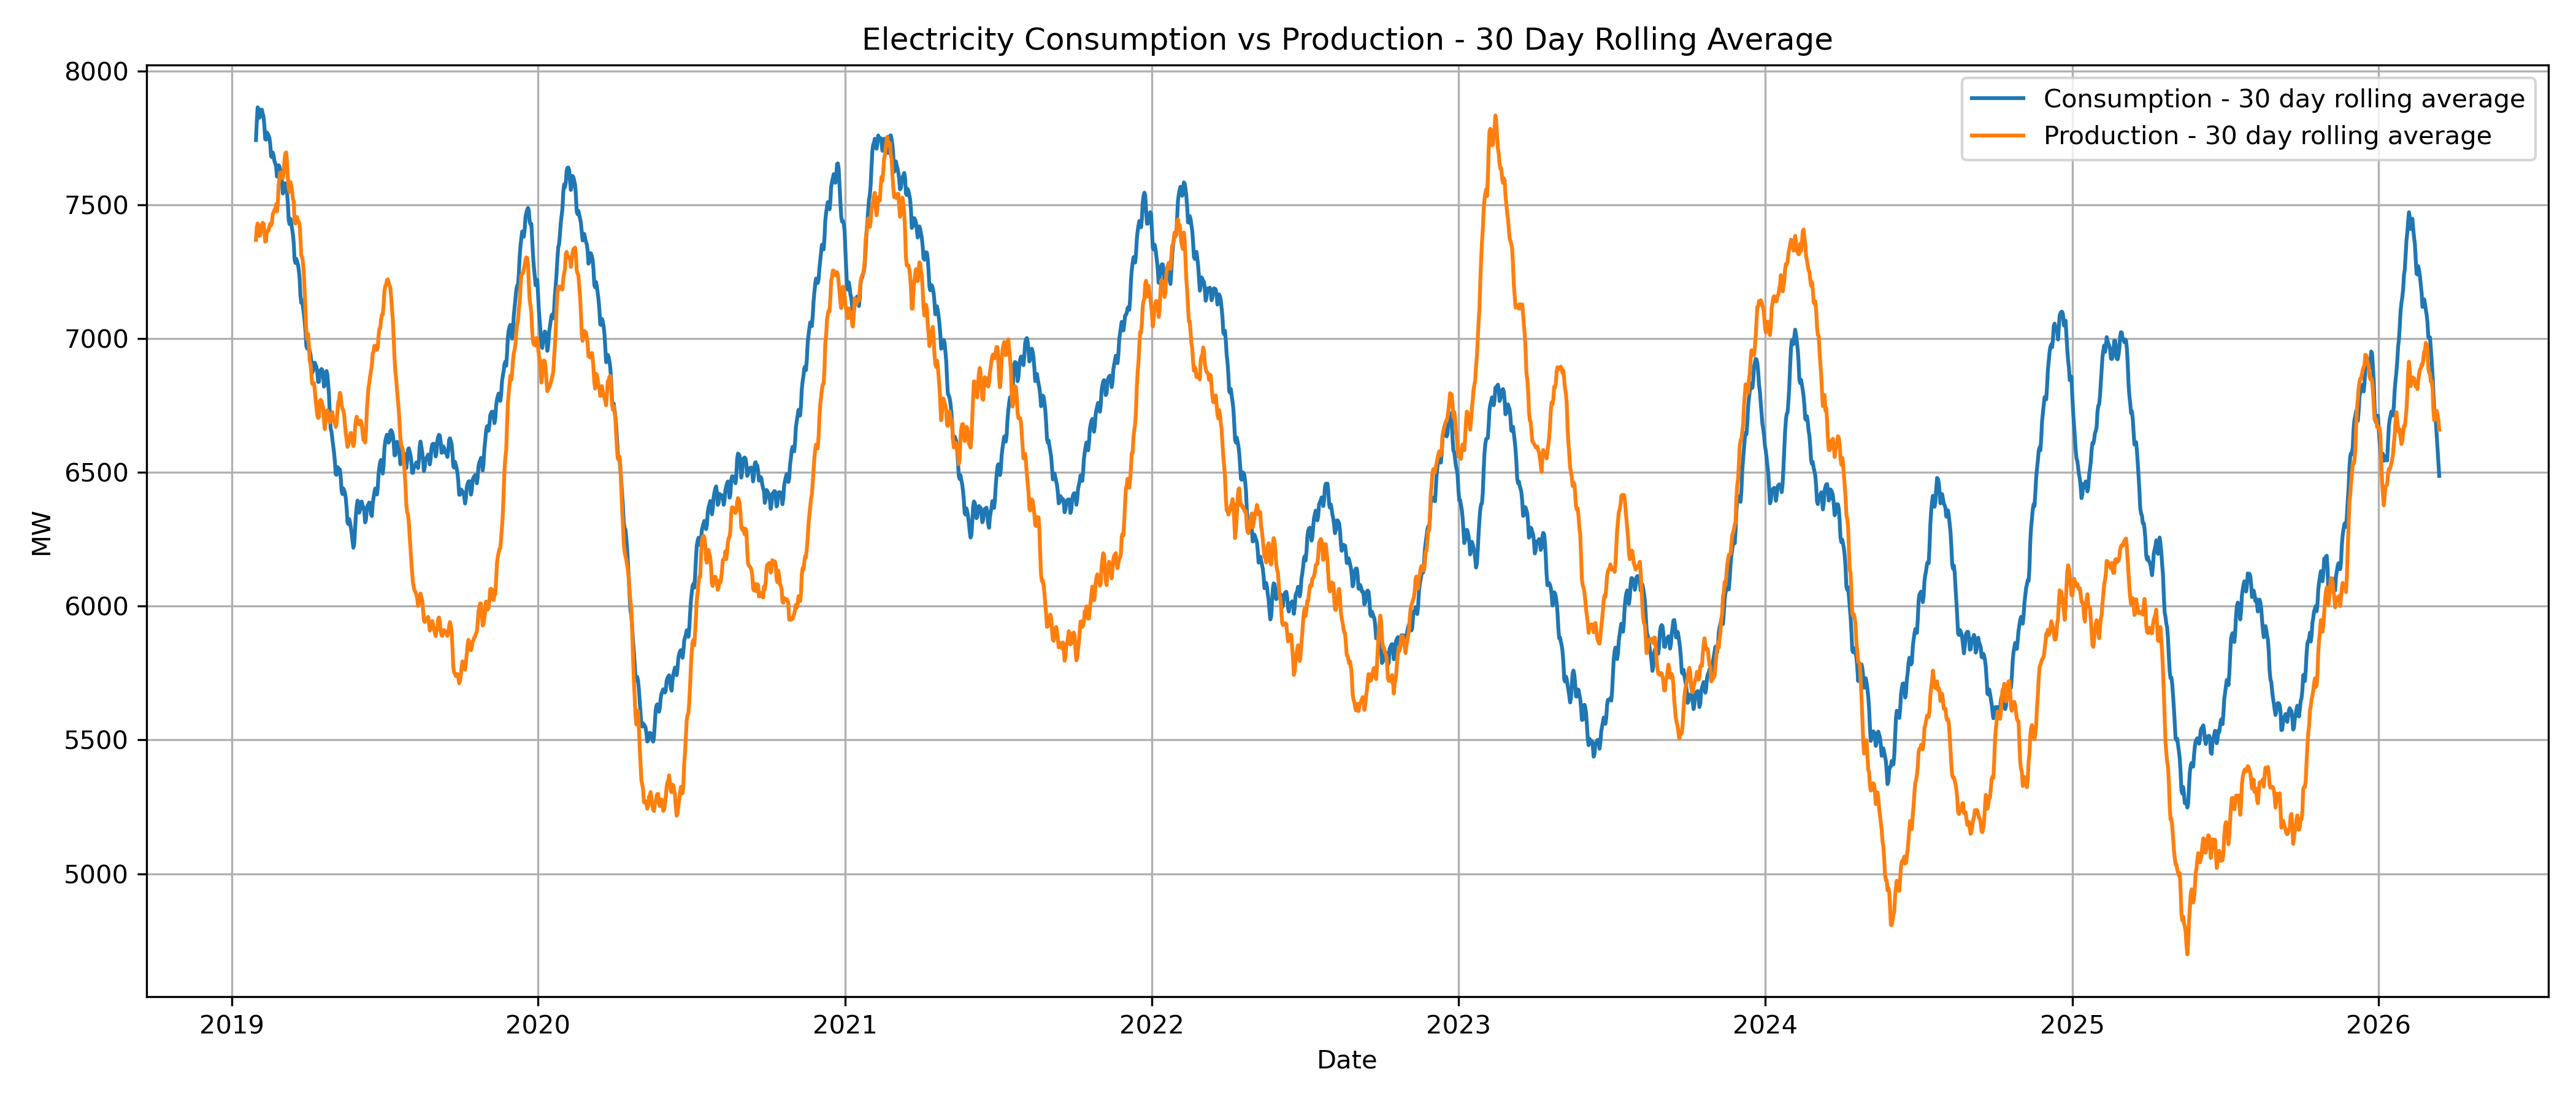
\includegraphics[width=\linewidth]{../figures/figure1_consumption_vs_production_rolling.png}
\caption{Electricity consumption and production represented as 30-day rolling averages between 2019 and 2026.}
\label{fig:consumption-production}
\end{figure}

\subsection{Hourly and Weekly Consumption Patterns}

Figure~\ref{fig:consumption-heatmap} shows the average electricity consumption grouped by day of week and hour of day. The heatmap reveals a clear daily pattern: consumption is lowest during nighttime and early morning hours, especially between 00:00 and 05:00. After 06:00, demand increases rapidly and remains high throughout the day.

The highest average consumption values appear mainly during weekday evenings. The figure also shows that weekend consumption is visibly lower than weekday consumption. Sunday presents the lowest overall demand pattern, while Tuesday, Wednesday, and Thursday show some of the highest average values. This indicates that electricity consumption is strongly connected to human and economic activity schedules.

\begin{figure}[h]
\centering
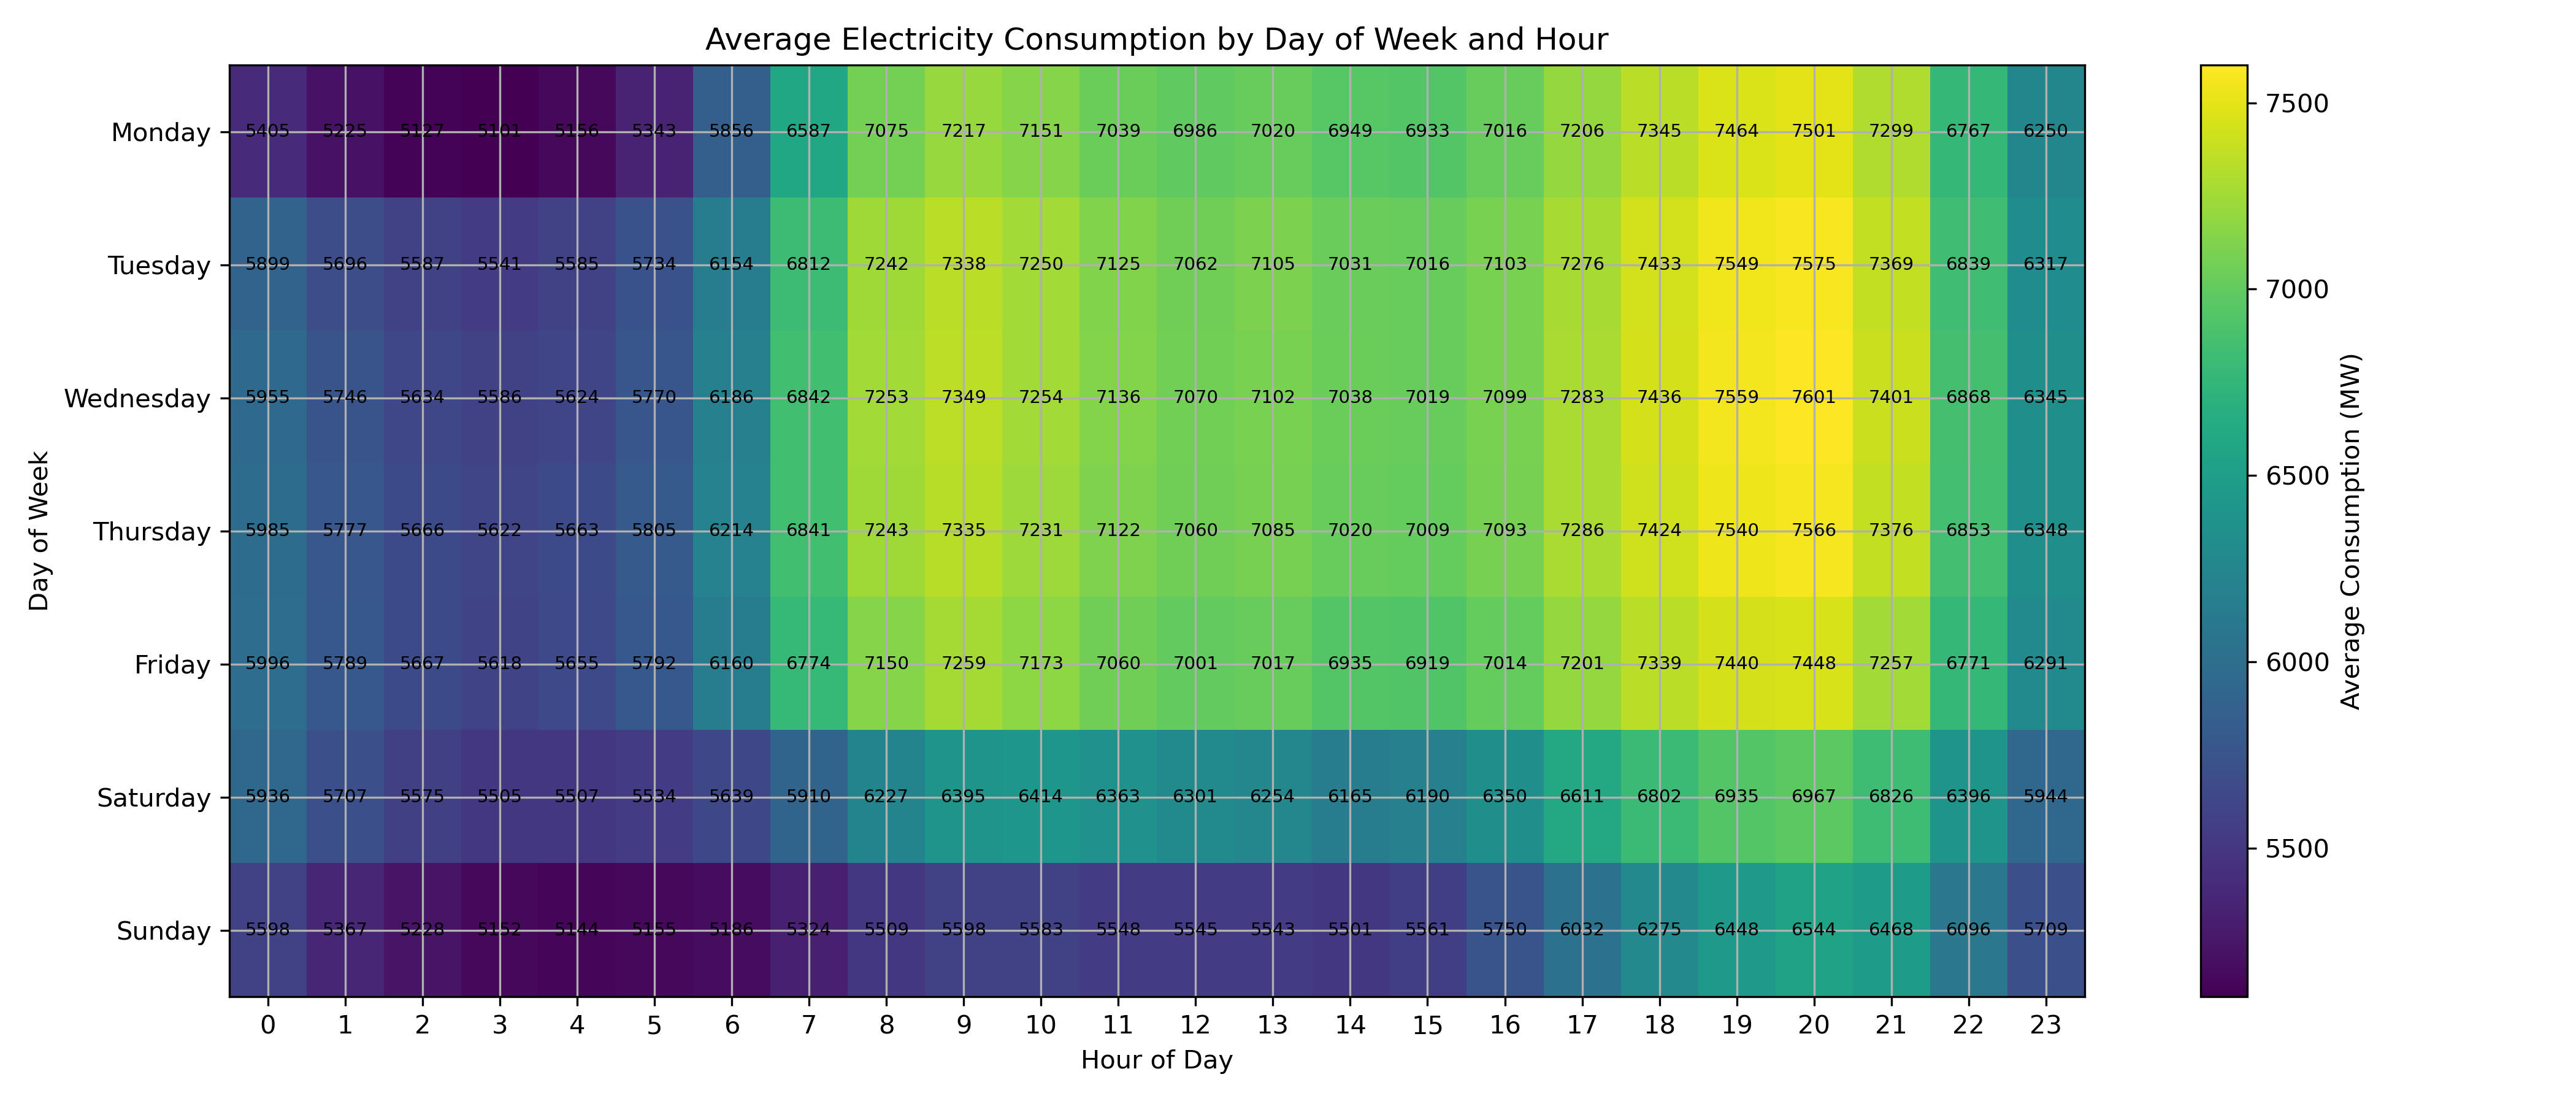
\includegraphics[width=\linewidth]{../figures/figure2_consumption_heatmap.png}
\caption{Average electricity consumption by day of week and hour of day.}
\label{fig:consumption-heatmap}
\end{figure}

\subsection{Electricity Production Mix}

Figure~\ref{fig:production-mix} illustrates the monthly average electricity production mix by source. The stacked area chart shows that Romania's electricity production is composed of several major sources, including nuclear, wind, hydroelectric, oil and gas, coal, solar, and biomass.

Nuclear production appears relatively stable across time, acting as a baseline source in the production mix. In contrast, hydroelectric, wind, coal, and oil and gas display stronger temporal variation. Solar and biomass have smaller contributions compared with the other sources. The figure shows that the electricity production mix is dynamic and changes noticeably from month to month.

This visualization is useful because it does not only show total production, but also how total production is built from individual sources. Therefore, it provides a more detailed view of the energy system than a simple production line plot.

\begin{figure}[h]
\centering
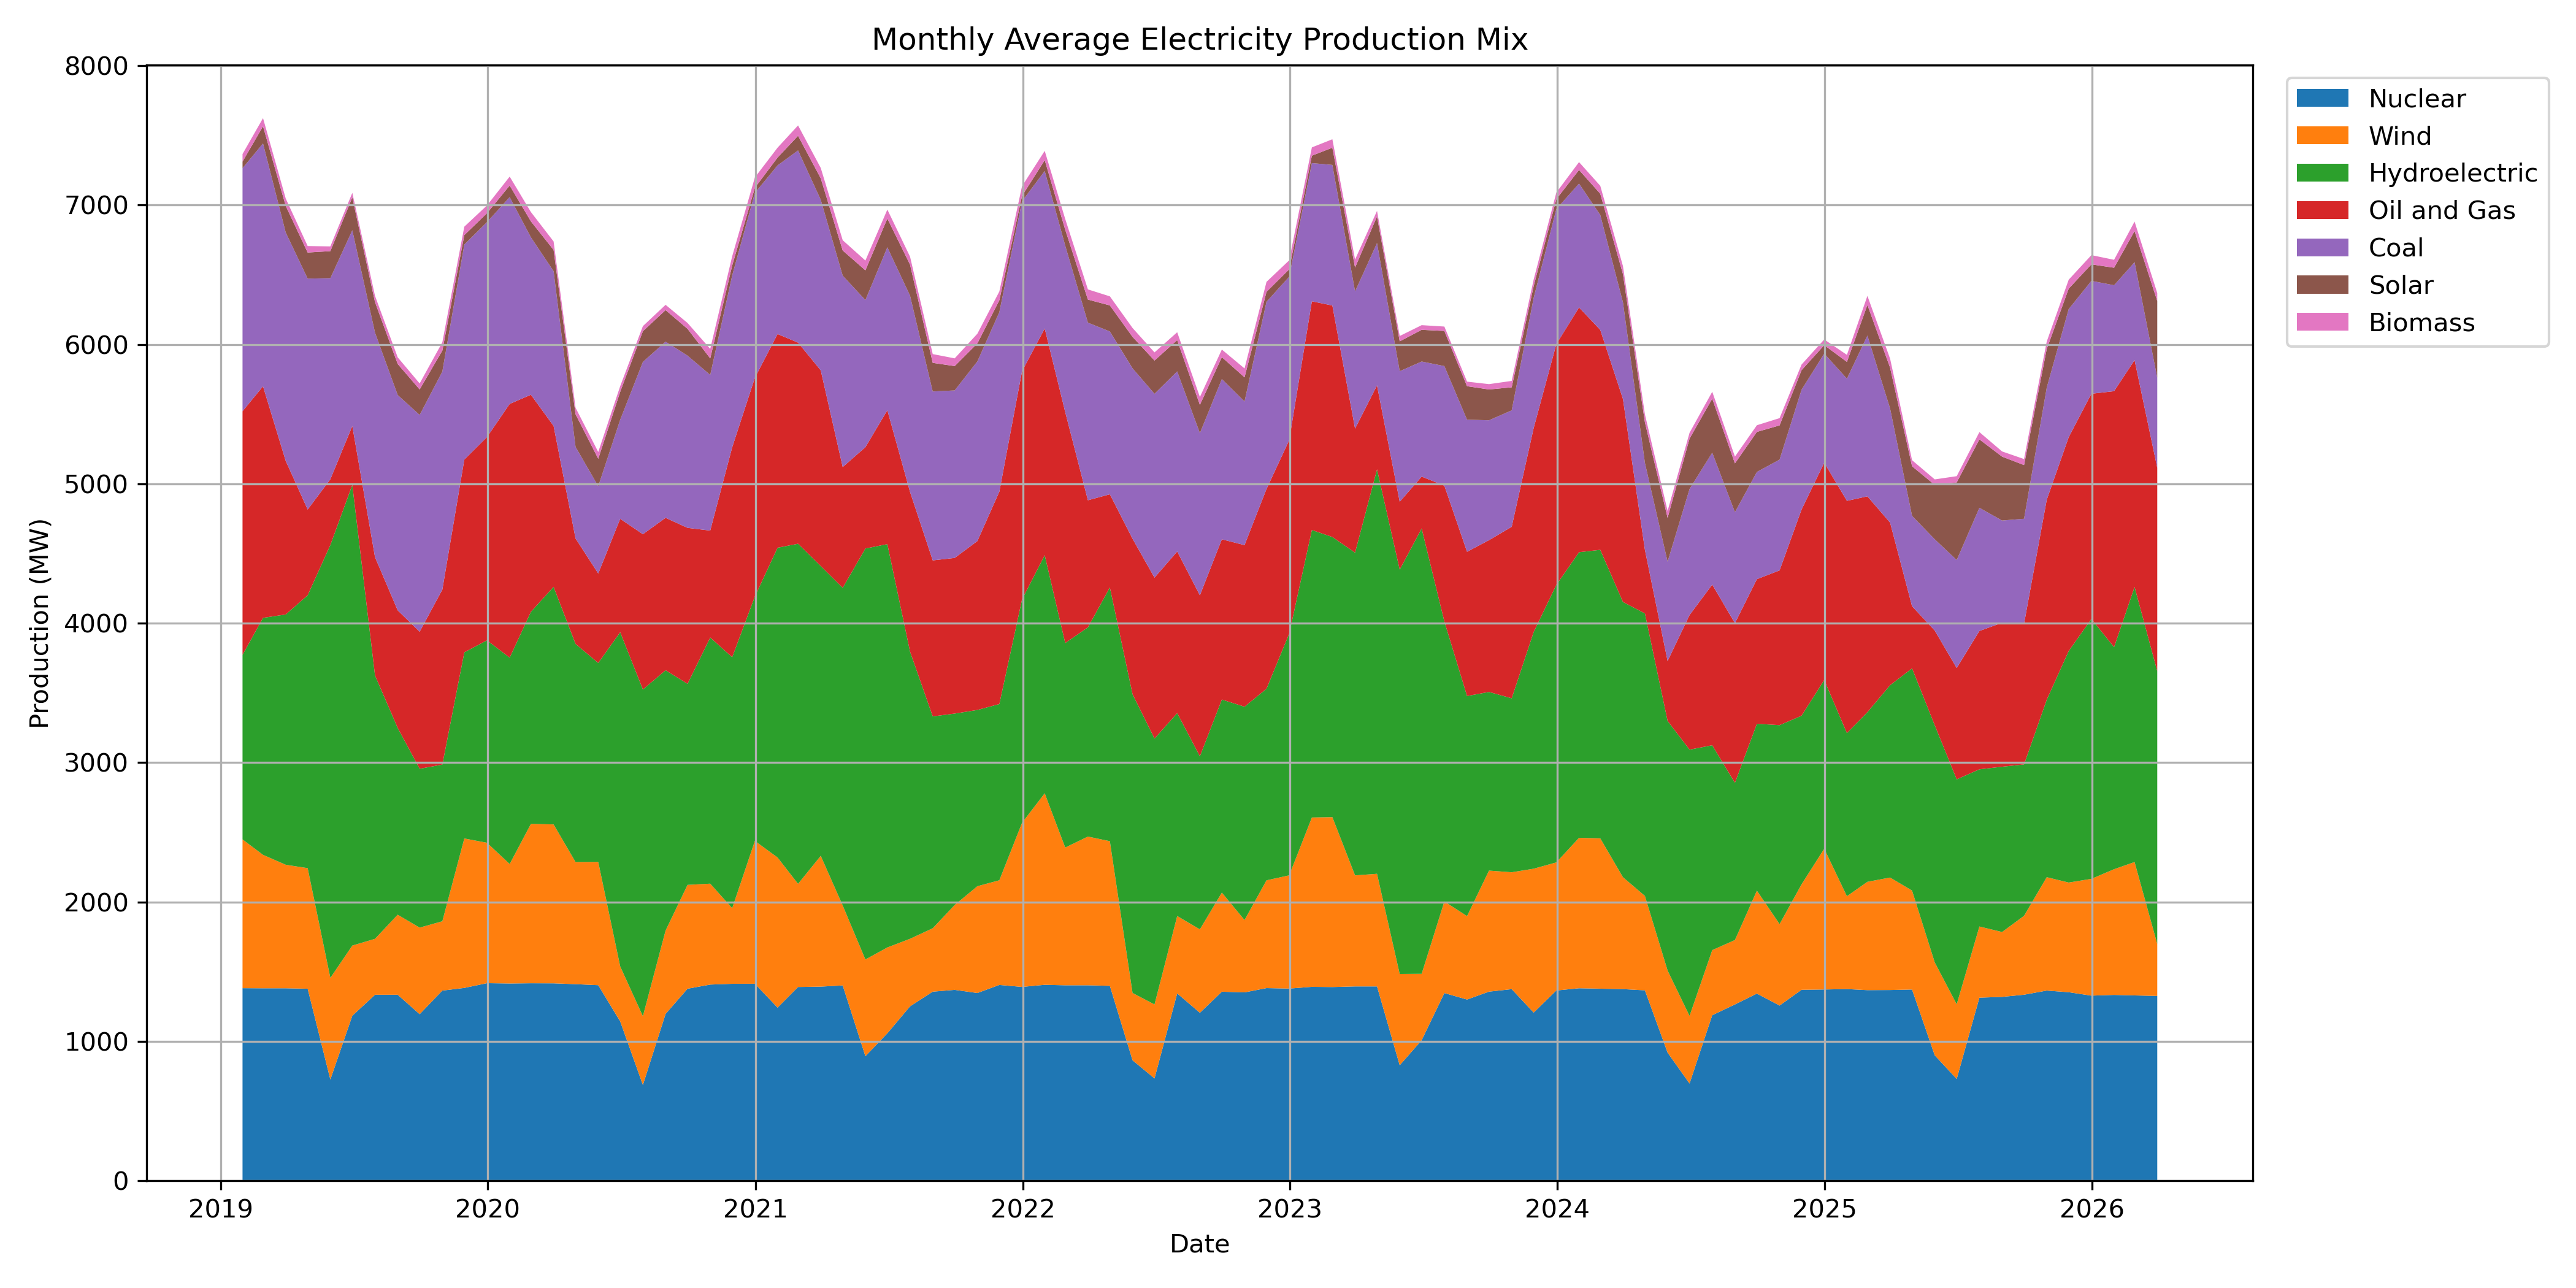
\includegraphics[width=\linewidth]{../figures/figure3_production_mix.png}
\caption{Monthly average electricity production mix by source.}
\label{fig:production-mix}
\end{figure}

\subsection{Monthly Consumption Distribution}

Figure~\ref{fig:monthly-boxplot} presents the monthly distribution of electricity consumption using boxplots. The figure reveals clear seasonal differences in demand. The highest median consumption values are observed during colder months, especially January, February, November, and December. Lower median values appear during spring and summer months.

The spread of the boxplots also differs across months, showing that electricity demand is more variable in some periods than others. Several outliers are visible, indicating unusual episodes of very high or very low consumption within specific months. These outliers are important because they show that even within the same month, consumption can sometimes deviate substantially from typical values.

\begin{figure}[h]
\centering
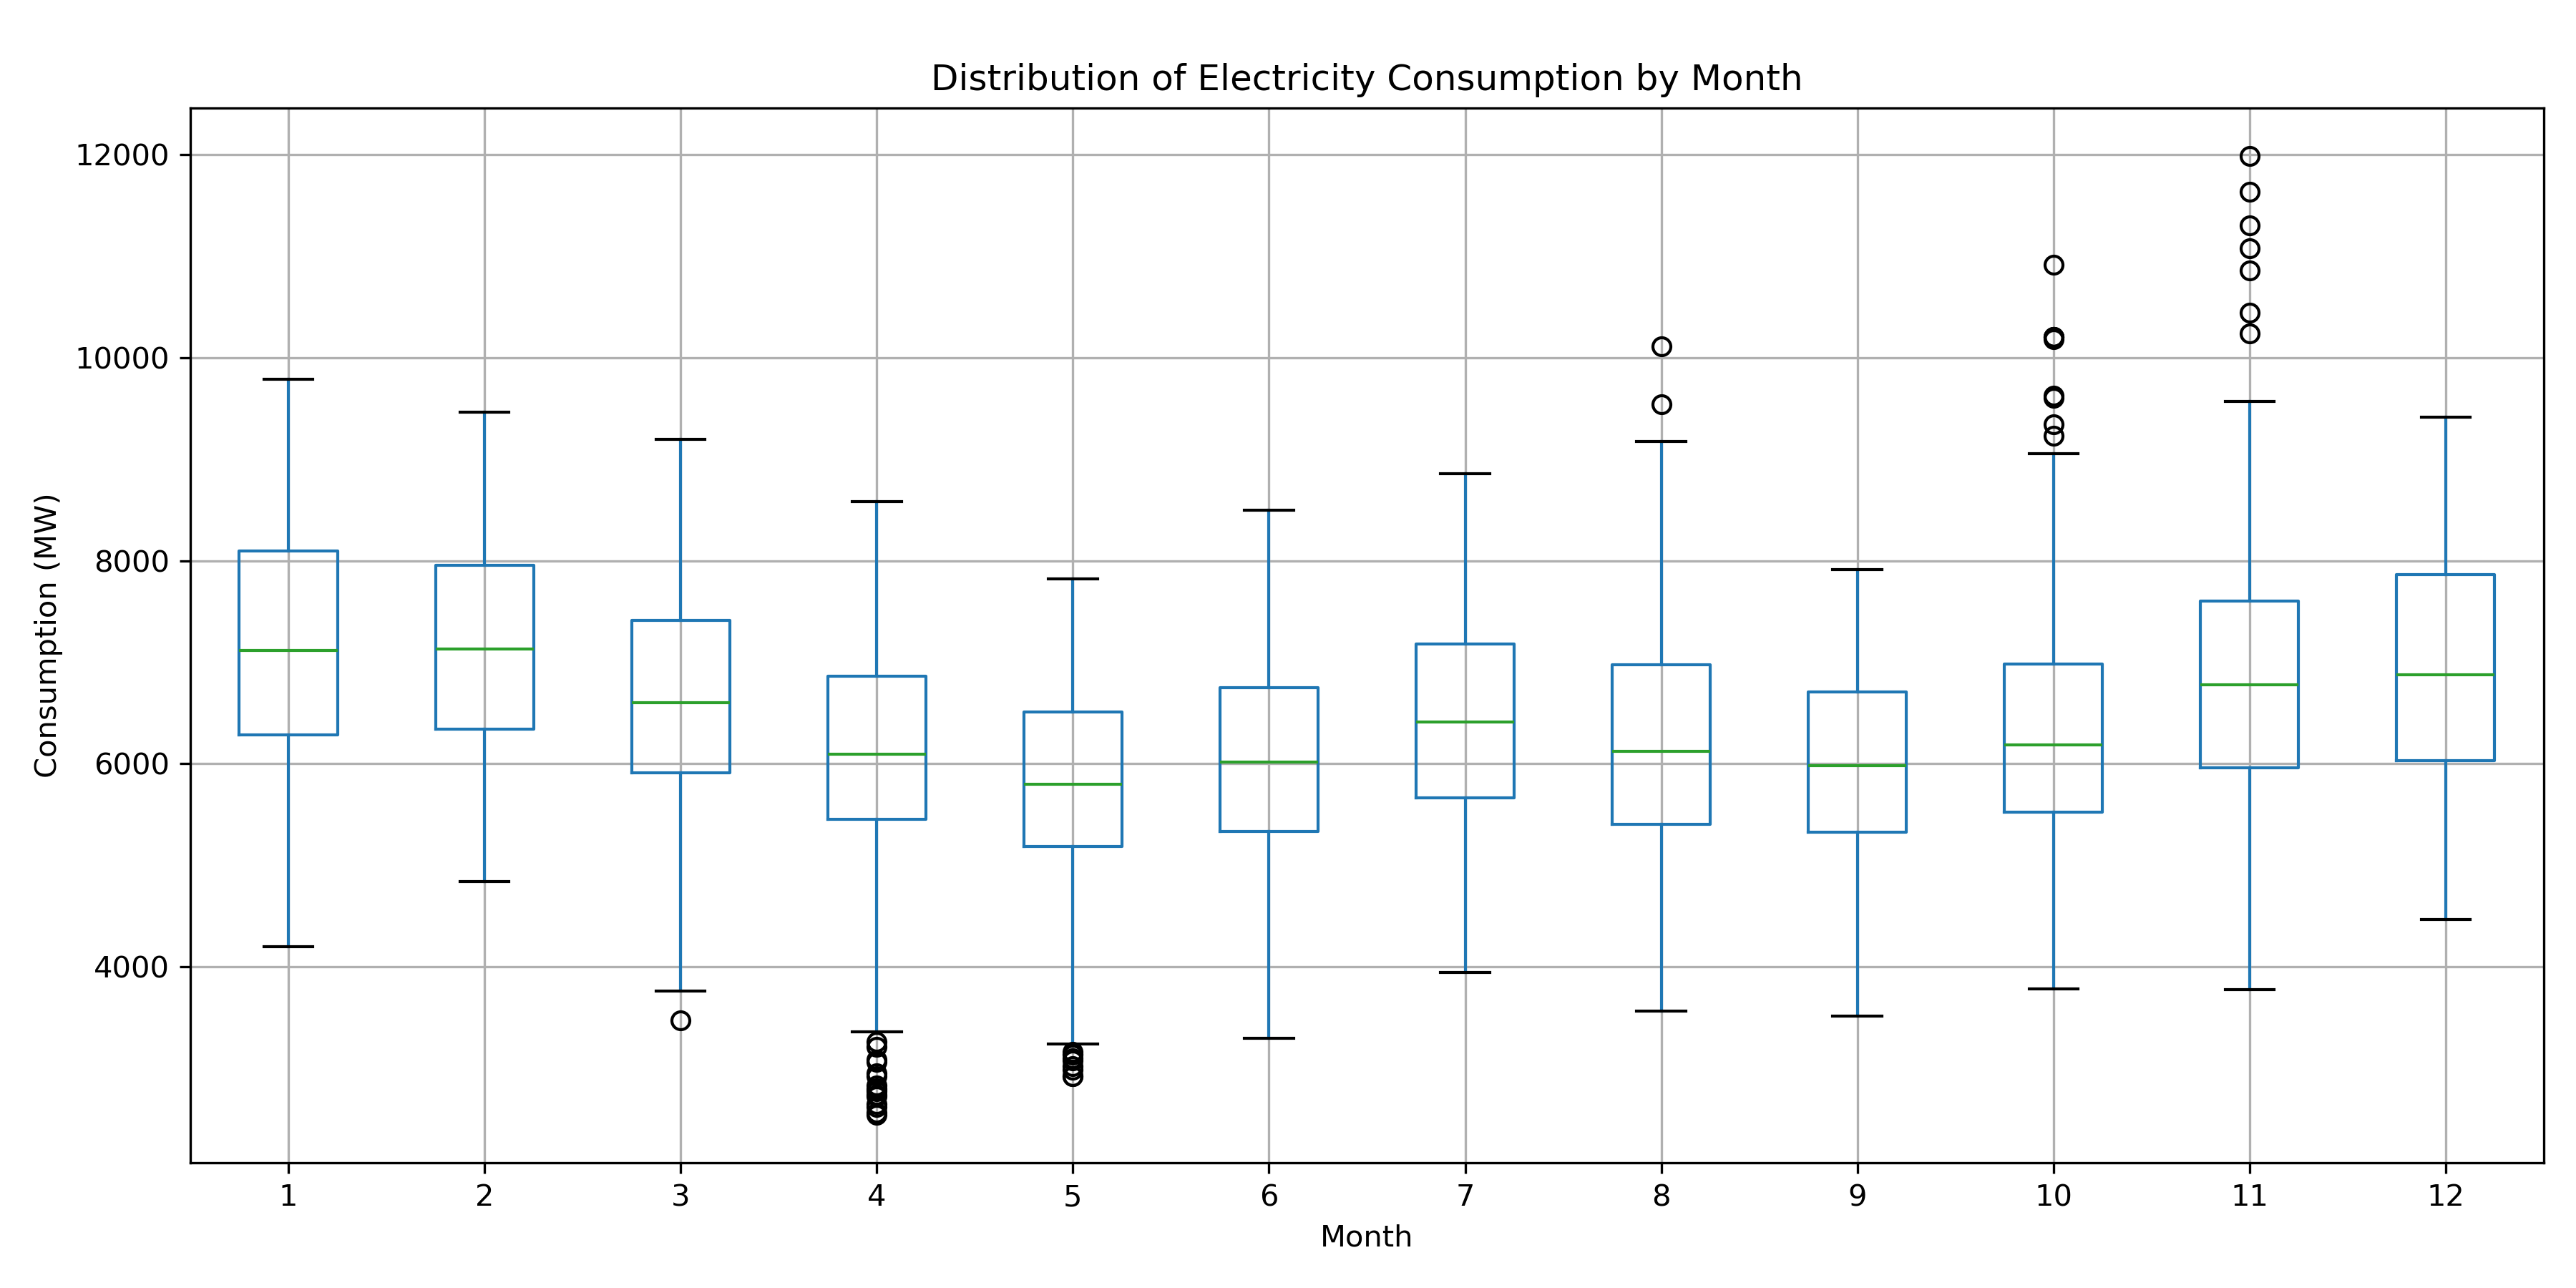
\includegraphics[width=\linewidth]{../figures/figure4_monthly_consumption_boxplot.png}
\caption{Monthly distribution of electricity consumption.}
\label{fig:monthly-boxplot}
\end{figure}

\subsection{Correlation Between Electricity Variables}

Figure~\ref{fig:correlation-matrix} shows the correlation matrix between the main electricity variables. Consumption and production are positively correlated, with a correlation coefficient of 0.69. This means that production generally increases when consumption increases.

Production is strongly correlated with renewable generation, while fossil generation is strongly associated with oil and gas and coal. Consumption is more strongly correlated with fossil sources than with renewable sources, suggesting that fossil generation plays an important role in supporting demand. The matrix also shows a positive relationship between renewable generation and the production-consumption balance.

The correlation matrix provides a compact summary of the relationships between variables. It helps identify which energy sources are more closely connected to total production and which sources are more related to consumption or balance.

\begin{figure}[h]
\centering
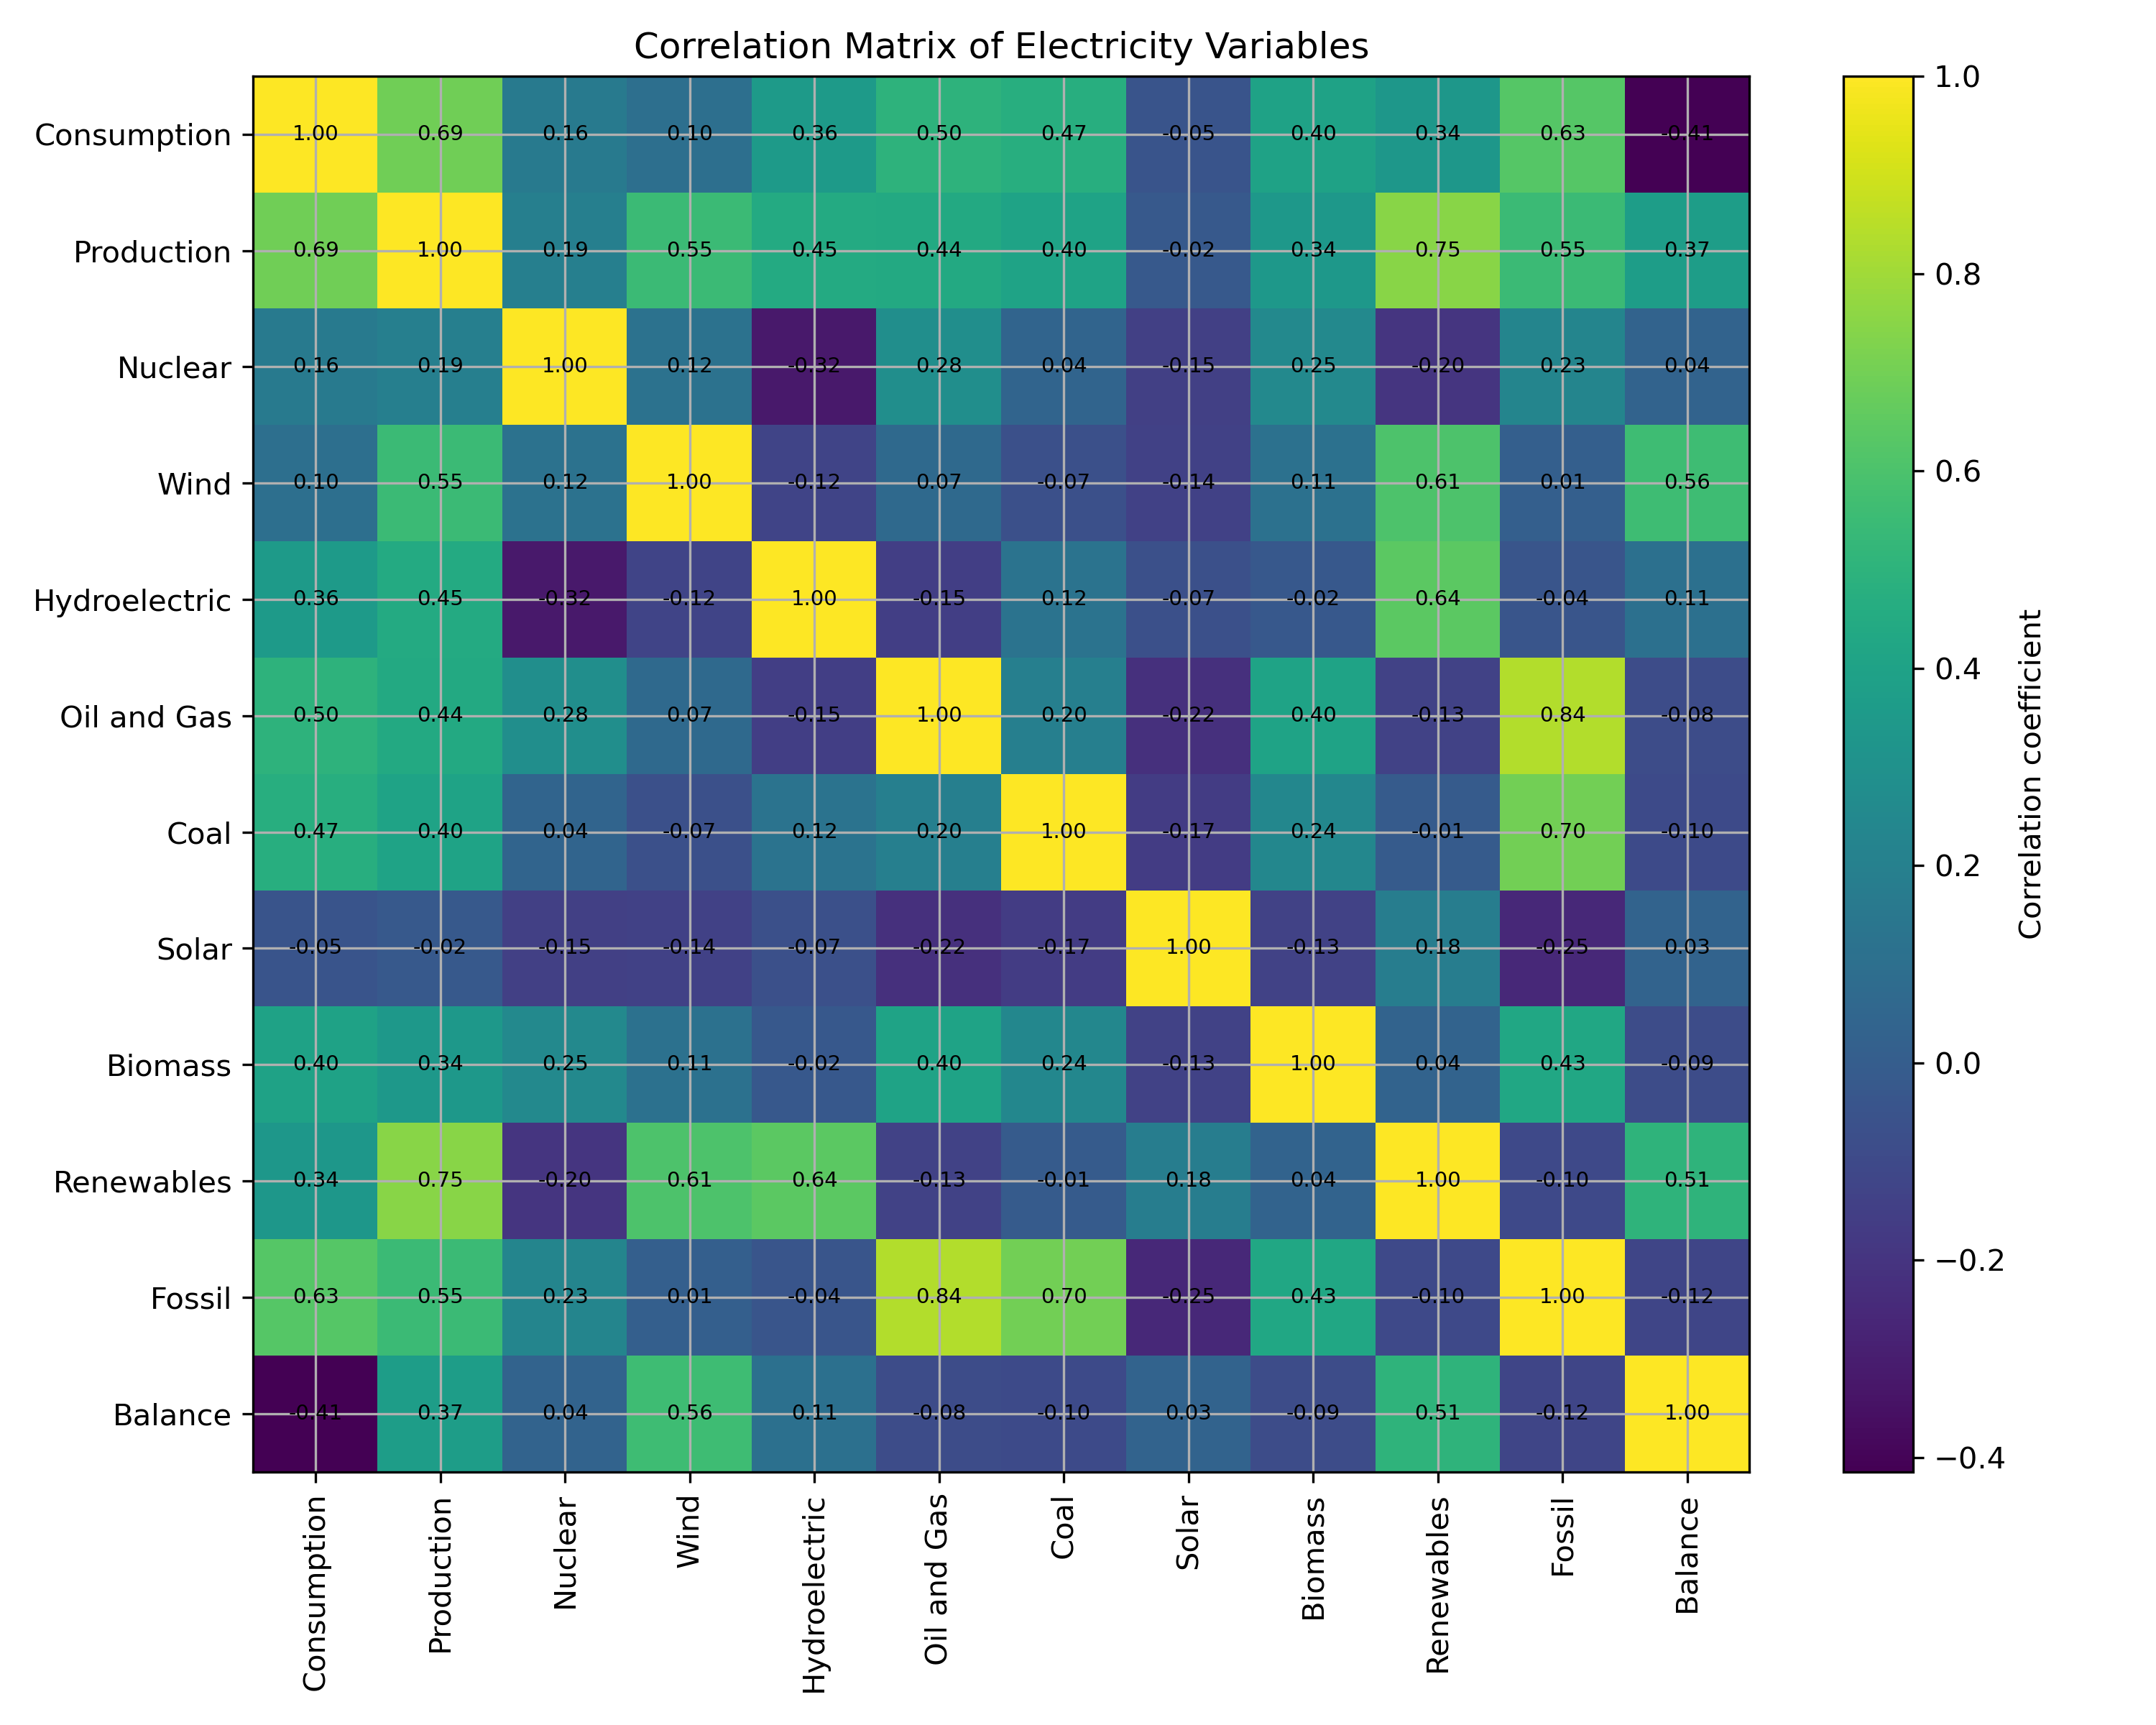
\includegraphics[width=\linewidth]{../figures/figure5_correlation_heatmap.png}
\caption{Correlation matrix of the main electricity variables.}
\label{fig:correlation-matrix}
\end{figure}

\subsection{Renewable vs Fossil Share}

Figure~\ref{fig:renewable-fossil-share} compares the monthly average share of renewable and fossil sources in total electricity production. Renewable sources generally account for a larger share of production than fossil sources, although both components vary substantially over time.

The figure also suggests a complementary relationship between the two categories: when the renewable share increases, the fossil share often decreases, and vice versa. This indicates that fossil sources may compensate for periods of lower renewable output, while renewable sources can reduce the relative dependence on fossil generation during favorable periods.

This figure complements the production mix chart because it summarizes the energy sources into two broader categories. As a result, it makes the renewable-fossil relationship easier to observe.

\begin{figure}[h]
\centering
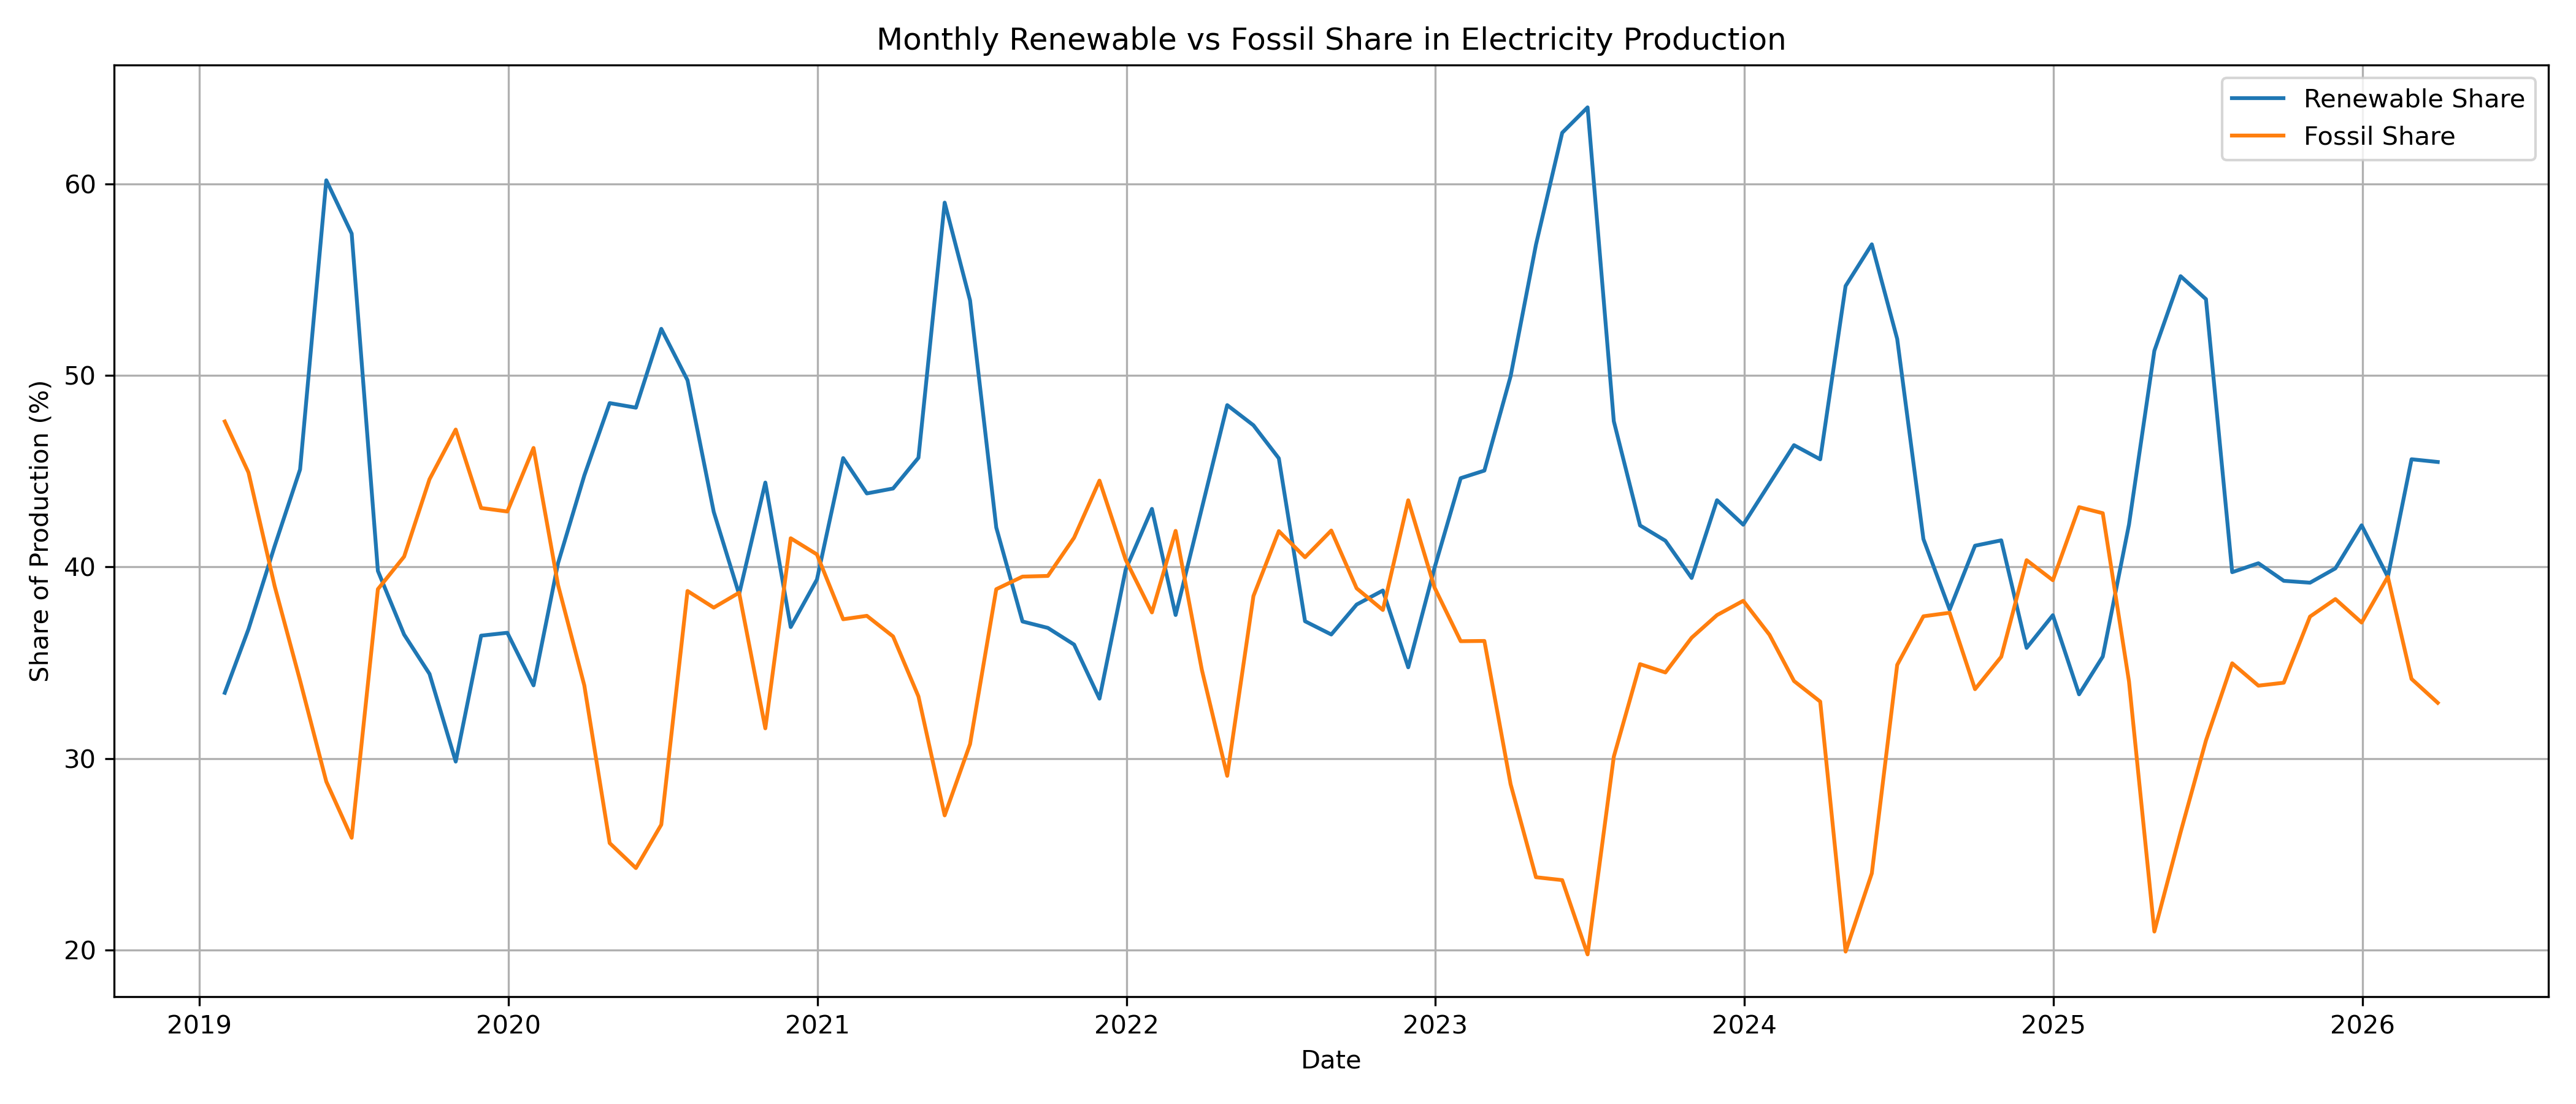
\includegraphics[width=\linewidth]{../figures/figure6_renewable_vs_fossil_share.png}
\caption{Monthly average share of renewable and fossil sources in total electricity production.}
\label{fig:renewable-fossil-share}
\end{figure}

\section{Discussion}

The visual analysis shows that Romania's electricity consumption has strong temporal patterns. Demand changes across years, months, days of the week, and hours of the day. The heatmap shows that electricity demand is strongly connected to daily activity, with low demand during nighttime hours and higher demand during daytime and evening hours. This pattern is expected because industrial, commercial, and household activities are more intense during the day.

The boxplot analysis confirms that seasonality is also important. Consumption tends to be higher during colder months, especially in winter and late autumn. This may be related to heating needs, lighting requirements, and changes in economic activity. The lower median consumption values observed during warmer months suggest that electricity demand is not uniform throughout the year.

The production mix analysis shows that Romania relies on a combination of stable and variable energy sources. Nuclear energy provides a relatively constant baseline, while hydroelectric, wind, coal, and oil and gas vary more strongly over time. This distinction between stable and variable sources is important because electricity systems must continuously balance production and consumption.

Renewable sources represent an important part of the electricity mix. Hydroelectric and wind generation appear to contribute strongly to renewable production, while solar and biomass have smaller shares. However, renewable generation is not constant. It varies across time, which means that the system still requires other sources to compensate for periods of lower renewable output.

The correlation analysis supports this interpretation. Consumption is positively correlated with production, which indicates that production generally follows demand. At the same time, consumption is more strongly correlated with fossil generation than with renewable generation. This suggests that fossil sources continue to play an important balancing role, especially when demand is high or renewable output is lower.

The comparison between renewable and fossil shares further strengthens this conclusion. Renewable sources often account for a larger share of production than fossil sources, but the inverse movement between the two categories suggests a compensatory relationship. When renewable share decreases, fossil share often increases. This does not necessarily imply causation, but it is an important visual pattern that describes the behavior of the energy mix.

Overall, the project demonstrates that big data visualization can transform a large hourly dataset into a clear and interpretable story. Instead of only observing raw numerical values, visualization makes it possible to identify demand peaks, seasonal patterns, production structure, and relationships between energy sources.

\section{Limitations and Future Work}

This project has several limitations. First, the analysis is mainly descriptive and visual. It identifies patterns and relationships, but it does not build predictive models for future electricity consumption or production. Second, the dataset contains electricity variables but does not include external factors such as temperature, weather conditions, holidays, industrial activity, or electricity prices. Including such variables could improve the interpretation of consumption and production patterns.

Another limitation is that correlation does not imply causation. The correlation matrix shows linear relationships between variables, but it cannot prove that one variable directly causes changes in another. For example, the relationship between fossil generation and consumption may be influenced by other factors that are not included in the dataset.

Future work could extend the analysis by combining this dataset with weather data, such as temperature, wind speed, precipitation, and solar radiation. This would make it possible to better explain the variation in renewable generation and electricity demand. Another possible extension would be to develop forecasting models for electricity consumption or renewable production. Finally, a more advanced network-based analysis could be created by modeling energy sources as nodes and correlations as edges, allowing the study of clusters and relationships between production sources.

\section{Conclusions}

This project used big data visualization techniques to analyze Romania's hourly electricity consumption and production patterns between 2019 and 2026. The analysis included temporal trends, hourly and weekly patterns, production mix, monthly distributions, correlations, and renewable versus fossil shares.

The main findings are that electricity consumption is not uniform over time. It is highest during colder months and during weekday daytime or evening hours. Production generally follows demand, but temporary differences between production and consumption are visible. The electricity production mix is dynamic, combining stable sources such as nuclear energy with more variable sources such as hydroelectric, wind, coal, and oil and gas.

Renewable sources represent an important part of Romania's electricity production, especially through hydroelectric and wind energy. However, fossil sources remain important for supporting demand and compensating for renewable variability. The visualizations show that the renewable and fossil components often move in opposite directions, suggesting that the energy system balances different sources depending on availability and demand.

Overall, the project shows how visualization can reveal patterns that are not immediately obvious from raw data. By using different types of plots, the analysis provides a coherent story about electricity demand, production structure, seasonality, and the relationship between renewable and fossil energy sources.

\bibliographystyle{IEEEtran}
\bibliography{references}

\end{document}
